% Copyright 2004 by Till Tantau <tantau@users.sourceforge.net>.
%
% In principle, this file can be redistributed and/or modified under
% the terms of the GNU Public License, version 2.
%
% However, this file is supposed to be a template to be modified
% for your own needs. For this reason, if you use this file as a
% template and not specifically distribute it as part of a another
% package/program, I grant the extra permission to freely copy and
% modify this file as you see fit and even to delete this copyright
% notice. 

\documentclass{beamer}
\usepackage[utf8x]{inputenc}
\usepackage{graphicx}
\graphicspath{ {./image/} }

% There are many different themes available for Beamer. A comprehensive
% list with examples is given here:
% http://deic.uab.es/~iblanes/beamer_gallery/index_by_theme.html
% You can uncomment the themes below if you would like to use a different
% one:
%\usetheme{AnnArbor}
%\usetheme{Antibes}
%\usetheme{Bergen}
%\usetheme{Berkeley}
%\usetheme{Berlin}
%\usetheme{Boadilla}
%\usetheme{boxes}
%\usetheme{CambridgeUS}
%\usetheme{Copenhagen}
%\usetheme{Darmstadt}
%\usetheme{default}
%\usetheme{Frankfurt}
%\usetheme{Goettingen}
%\usetheme{Hannover}
\usetheme{Ilmenau}
%\usetheme{JuanLesPins}
%\usetheme{Luebeck}
%\usetheme{Madrid}
%\usetheme{Malmoe}
%\usetheme{Marburg}
%\usetheme{Montpellier}
%\usetheme{PaloAlto}
%\usetheme{Pittsburgh}
%\usetheme{Rochester}
%\usetheme{Singapore}
%\usetheme{Szeged}
%\usetheme{Warsaw}

\title{Projet système\\Master 1}

% A subtitle is optional and this may be deleted

\author{R. Blanc \and A.Castel \and C.Eymond Laritaz \and M.Garnier}
% - Give the names in the same order as the appear in the paper.
% - Use the \inst{?} command only if the authors have different
%   affiliation.

\institute[Université Grenoble Alpes] % (optional, but mostly needed)
{
  UFR IM²AG\\
  Université Grenoble Alpes
}
% - Use the \inst command only if there are several affiliations.
% - Keep it simple, no one is interested in your street address.

\date{Jeudi 17 Janvier 2019}
% - Either use conference name or its abbreviation.
% - Not really informative to the audience, more for people (including
%   yourself) who are reading the slides online

% logo of my university
%\titlegraphic{
 %{\centering
 %\vspace{-1.5cm}
 %\includegraphics[height=1cm]{logoUnQuart}\hspace*{6.5cm}~%
 %\includegraphics[height=1cm]{logo_im2ag}
 %}
%}

\subject{Informatique}
% This is only inserted into the PDF information catalog. Can be left
% out. 

% If you have a file called "university-logo-filename.xxx", where xxx
% is a graphic format that can be processed by latex or pdflatex,
% resp., then you can add a logo as follows:

%\pgfdeclareimage[height=0.7cm]{team-logo}{logo_team.png}
%\logo{\pgfuseimage{team-logo}}

% Delete this, if you do not want the table of contents to pop up at
% the beginning of each subsection:
\AtBeginSubsection[]
{
  \begin{frame}<beamer>{}
    \tableofcontents[currentsection,currentsubsection]
  \end{frame}
}

% Let's get started
\begin{document}

\begin{frame}
  \titlepage
\end{frame}

\begin{frame}{Outline}
  \tableofcontents%[pausesections]
  % You might wish to add the option [pausesections]
\end{frame}

% Section and subsections will appear in the presentation overview
% and table of contents.

\section{Nachos Input-Output}
\subsection{Appels systèmes et choix d’implémentations }
\begin{frame}
	\begin{block}{Appels systèmes}
		\begin{itemize}
			\item void PutChar(char c);
			\item void PutString(char *s);
			\item char GetChar();
			\item void GetString(char *s, int n);
			\item void PutInt(int n);
			\item void GetInt(int *n);
		\end{itemize}
	\end{block}
	\begin{block}{Choix d’implémentation}
		\begin{itemize}
			\item Limite de chaîne de caractères traités de 200
			\item Les espaces sont lus comme les autres caractères 
		\end{itemize}		
	\end{block}
\end{frame}







\section{Multi-Threading}
\subsection{Gestion de la pile}
\begin{frame}
	\begin{block}{Choix d’implémentation }
		\begin{itemize}
			\item L'emplacement dans la pile des Threads est géré avec une Bitmap
			\item 3 pages sont allouées à chaque Thread utilisateur 
			\item La valeur maximale de SP que le main peut atteindre est fixée 
			\item Le Thread Main n’apparaît pas dans la Bitmap
		\end{itemize}
	\end{block}
\end{frame}

\begin{frame}
  	\begin{center}
	  	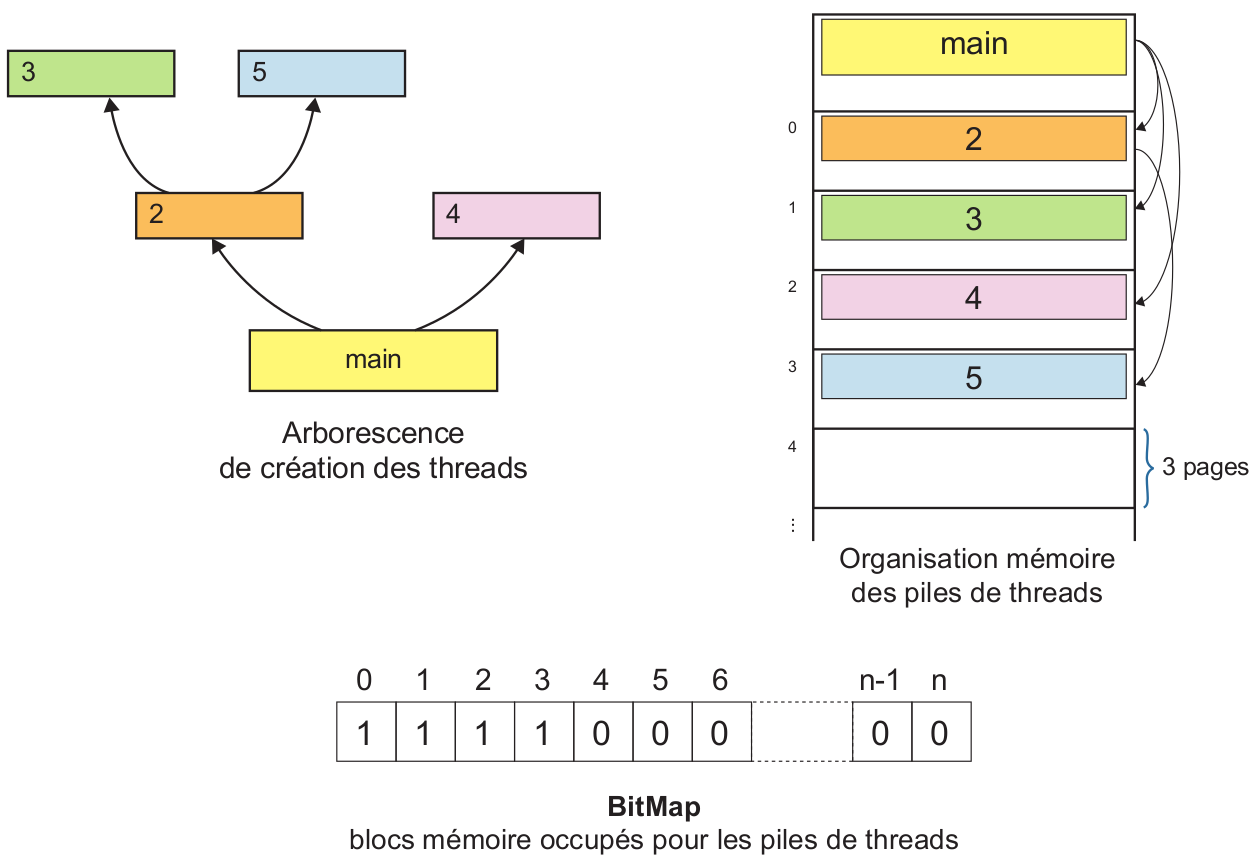
\includegraphics[scale=0.23]{images/FS3.png}
  	\end{center}
\end{frame}

\begin{frame}
  	\begin{center}
	  	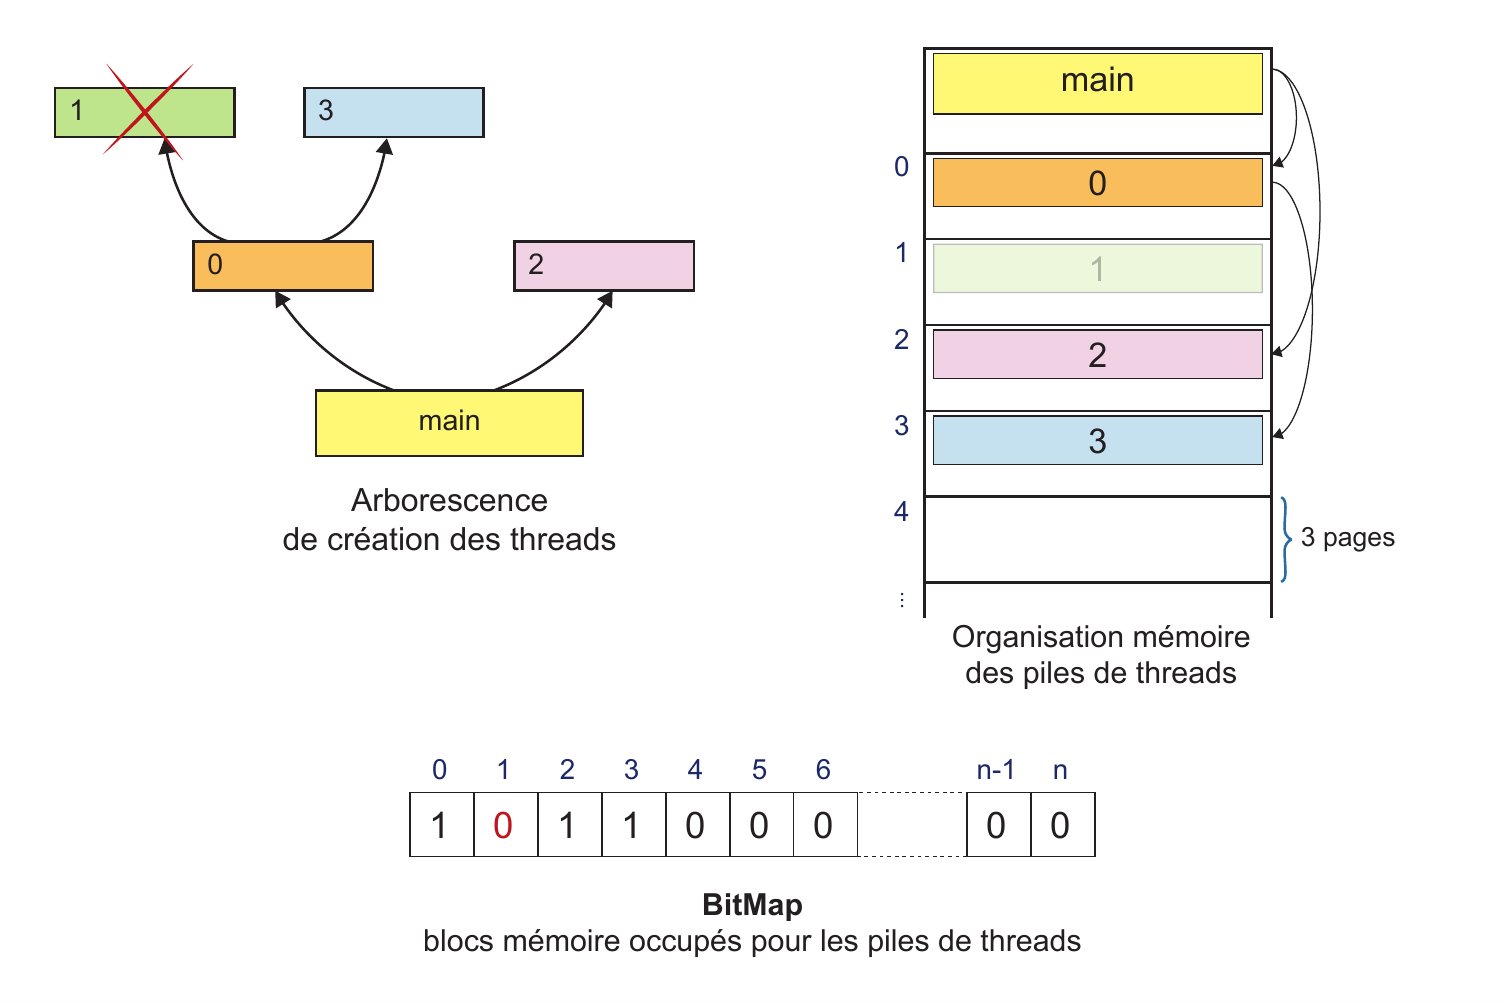
\includegraphics[scale=0.23]{images/FS4.png}
  	\end{center}
\end{frame}

\begin{frame}
  	\begin{center}
	  	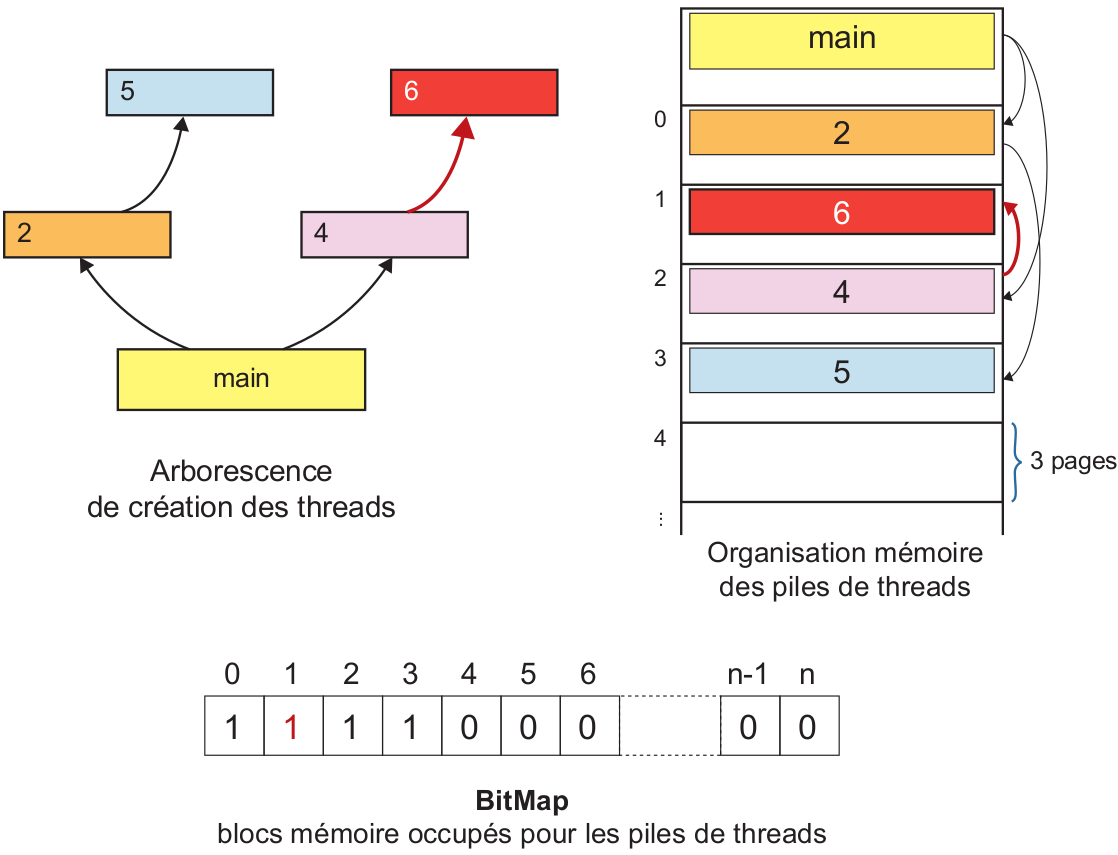
\includegraphics[scale=0.25]{images/FS5.png}
  	\end{center}
\end{frame}


\subsection{Appels Système}
\begin{frame}
	\begin{block}{Appels systèmes}
		\begin{itemize}
			\item<1-> int UserThreadCreate(void f(void *arg), void *arg);
			\begin{itemize}
				\item<1-> Créé un Thread utilisateur, qui exécute la fonction "f" avec les arguments "arg"
				\item<1-> Retourne l'identifiant du Thread créé
			\end{itemize}
			\item<2-> void UserThreadExit();
			\begin{itemize}
				\item<1-> Termine un Thread utilisateur
			\end{itemize}
			\item<3-> void UserThreadJoin(int tid);
			\begin{itemize}
				\item<1-> Attend la terminaison du Thread utilisateur "tid"
			\end{itemize}
		\end{itemize}
	\end{block}
\end{frame}

\begin{frame}{Autres ajouts}
	\begin{block}{Synchronisation }
		\begin{itemize}
			\item<1-> Nouveau type \texttt{semaphore\_t} au niveau utilisateur, avec les appels systèmes qui permettent de le manipuler.
			\begin{itemize}
				\item<2-> semaphore\_t Sem\_Init(int nbJetons);
				\item<3-> int Sem\_P(semaphore\_t s);
				\item<4-> int Sem\_V(semaphore\_t s);
				\item<5-> int Sem\_GetValue(semaphore\_t s);
				\item<6-> int Sem\_Destroy(semaphore\_t s);
			\end{itemize}
			\item<7-> Fonctionnement avec une table de sémaphores noyau
		\end{itemize}
	\end{block}
\end{frame}

\begin{frame}
	\begin{block}{Choix d’implémentation }
		\begin{itemize}[<+->]
			\item Le nombre de Threads est limité à 50 
			\item La gestion de la terminaison des Threads est laissée à l'utilisateur, sauf pour le main
			\item Un Thread peut faire un UserThreadJoin() sur n'importe quel Thread créé lors de l'exécution du programme
			\item L'identifiant d'un Thread est unique, il n'est jamais réutilisé
			\item C'est à l'utilisateur d'utiliser correctement UserThreadJoin() 
			\begin{itemize}
				\item Par exemple, l'utiliser sur un identifiant de Thread incorrect donnera lieu à un comportement indéfini.
			\end{itemize}			
		\end{itemize}
	\end{block}
\end{frame}

\section{Mémoire virtuelle}
\subsection{Mémoire virtuelle}
\begin{frame}{Pagination}
	\begin{block}{Mémoire virtuelle}
		\begin{itemize}[<+->]
			\item Frame Provider
			\item Politiques d'allocation
			\begin{itemize}
				\item FIRST\_FREE\_FRAME
				\item RANDOM\_FREE\_FRAME			
			\end{itemize}
		\end{itemize}
	\end{block}
\end{frame}
\subsection{Multiprocessus}

\begin{frame}{Multiprocessus}
	\begin{block}{Appel système}
		\begin{itemize}[<+->]
			\item Création d'un nouveau type utilisateur pid\_t
			\item pid\_t ForkExec(char* filename)
			\begin{itemize}
				\item<1-> Crée un nouveau processus qui exécute le programme contenu dans le fichier filename.
				\item<2-> Renvoie le pid\_t correspondant au nouveau processus
			\end{itemize}
			\item void waitpid(pid\_t p)
			\begin{itemize}
				\item<1-> Attend la terminaison du processus p
			\end{itemize}
		\end{itemize}
	\end{block}
\end{frame}

\section{Système de fichiers}
\subsection{Arborescence de répertoires}
\begin{frame}
  \begin{block}{Principe}
  	\begin{itemize}%[<+->]
  		\item Le secteur contenant l'i-node du répertoire Root est le 1
  		\item Un répertoire est représenté sur disque par un fichier Nachos classique
  	\end{itemize}  
  \end{block}
  \begin{center}
	  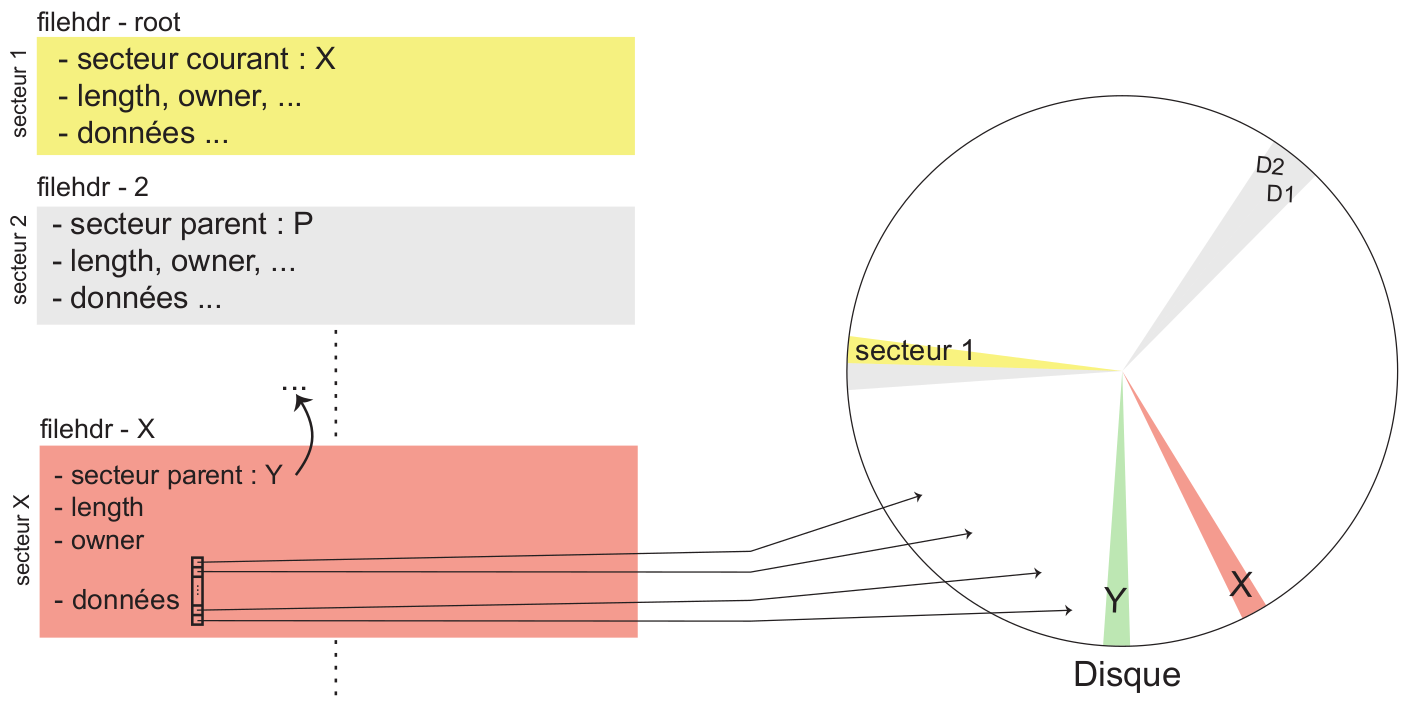
\includegraphics[scale=0.2]{images/FS1.png}
  \end{center}
\end{frame}

\begin{frame}
  \begin{block}{Fonctionnalités}
  	\begin{itemize}[<+->]
  		\item Création de répertoire (mkdir)
  		\begin{itemize}
  			\item Le nouveau répertoire contiendra deux fichiers : "." et ".."
  		\end{itemize}
  		\item Changement de répertoire courant (cd)
  		\begin{itemize}
  			\item Parcours de l'arborescence grâce aux fichiers spéciaux "." et ".."
  			\item Le répertoire racine s'appelle "/"
  		\end{itemize}
  	\end{itemize}
  \end{block}
\end{frame}
\subsection{Page des fichiers ouverts}


\begin{frame}
	\begin{block}{Appels systèmes}
		\begin{itemize}
			\item<1-> int Create (char *name, int size);
			\begin{itemize}
				\item<1->Retourne 1 si l'execution s'est bien passé, 0 sinon
				\item<1->Créé un fichier "name" dans le répertoire courant,de taille "size"
			\end{itemize}
			\item<2-> OpenFileId Open (char *name);
			\begin{itemize}
				\item<1->Ouvre le fichier "name", retourne un OpenFileId, manipulable par l'utilisateur
				\item<1->Renvoie -1 si l'ouverture est impossible
			\end{itemize}			
		\end{itemize}
	\end{block}
\end{frame}

\begin{frame}
	\begin{block}{Appels systèmes}
		\begin{itemize}
			\item<1-> int Write (char *buffer, int size, OpenFileId id);
			\begin{itemize}
				\item<1->Ecrit la chaine de taille "size" contenue dans "buffer" dans le fichier "id"
				\item<1->Renvoie le nombre de bytes effectivement écrits
			\end{itemize}
			\item<2-> int Read (char *buffer, int size, OpenFileId id);
			\begin{itemize}
				\item<1->Remplis "buffer" avec un nombre de caractères "size" lus depuis le fichier "id"
				\item<1->Renvoie le nombre de bytes lus
			\end{itemize}	
			\item<3-> void Close (OpenFileId id);
			\begin{itemize}
				\item<1->Ferme le fichier "id"
			\end{itemize}		
		\end{itemize}
	\end{block}
\end{frame}

\begin{frame}
	\begin{block}{Table des fichiers ouverts}
		\begin{itemize}
			\item<1-> Interface entre le système de fichiers et le programme utilisateur.
			\item<1-> Nachos permet l'ouverture de 10 fichiers simultanément au total au niveau des programmes utilisateurs
			\item<1-> Les indices 0 et 1 se sont jamais utilisés, ils sont réservés.
		\end{itemize}		
	\end{block}	
  	\begin{center}
	  	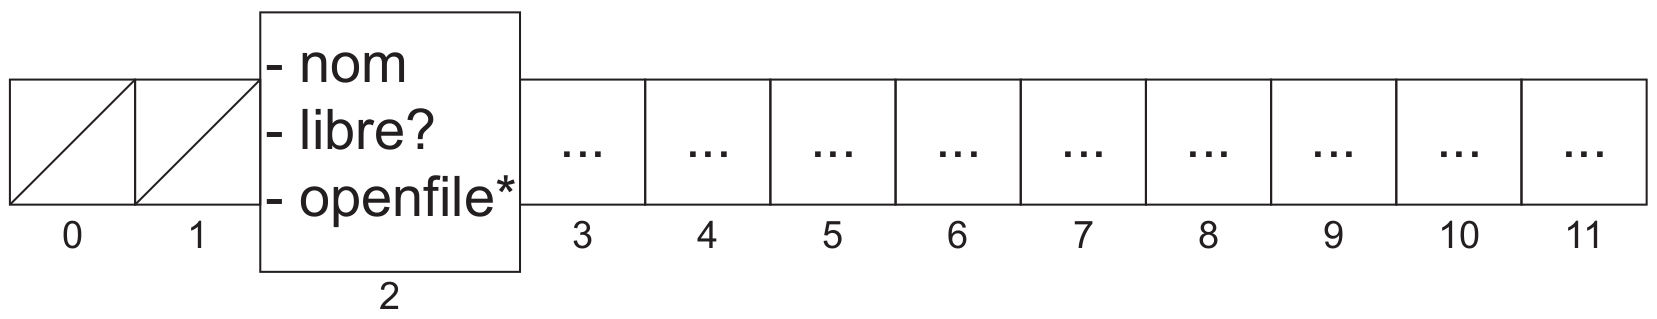
\includegraphics[scale=0.2]{images/FS2.png}
  	\end{center}	
\end{frame}

\end{document}

